\section{Tangent Lines and Instantaneous Rates of Change}
\label{sec:tangents}

\subsection{Tangent Line Concepts}

\begin{example} 
Suppose that Figure \ref{fig:2-2-bacteria} plots the population of a bacteria culture $t$ hours after an antibiotic is added to the culture. What is the rate at which the population  is changing eight hours after the bacteria is added to the culture?
\end{example}

\begin{figure}[ht!]
\centering
\begin{tikzpicture}[scale=1]
    % grid
    \draw[step=1, very thin, gray] (0, 0) grid (10, 6);

    % axes
    \draw[->] (-0.2,0) -- coordinate (x axis mid) (10.5,0) node[right] {$t$};
    \draw[->] (0,-0.2) -- coordinate (y axis mid) (0, 6.5) node[above] {$y$};

    % ticks
    \foreach \x in {1, 2, ..., 10}
     		\draw (\x,1pt) -- (\x,-3pt)
			node[anchor=north] {\x};
    	\foreach \y in {1, 2, ..., 6}
     		\draw (1pt,\y) -- (-3pt,\y) 
     			node[anchor=east] {\y}; 

    % labels
    \node[below = 15] at (x axis mid) {Time (hours)};
	\node[rotate=90, above = 25] at (y axis mid) {Bacteria population (millions)};

    % plot 
    \draw[smooth, samples=1000, domain=0:10.2, very thick, color=aldRed] plot(\x,{(6*\x+2)*exp(-\x/2)});    

    % points
    
    % legend

\end{tikzpicture}
\caption{Population of a bacteria culture $t$ hours after an antibiotic is added.}
\label{fig:2-2-bacteria}
\end{figure}

If we wanted to know the rate of change of the culture between two distinct points in time, then we could apply the techniques of the last section. Here, however, we want to know the rate of change at an instant in time, or the {\bf instantaneous rate of change}\index{Rate of change!instantaneous} of the culture at a single point in time. We found the average rate of change by computing the slope of a secant line. Here, we can estimate the instantaneous rate of change by approximating the slope of a certain line called a {\bf tangent line}\index{Line!tangent}\index{Tangent line} of the curve at a point. 

An informal definition of a tangent line of a curve is that a {\bf tangent line} of a curve is a line that touches one point on the curve in such a way that the curve and line would be indistinguishable if you zoomed in closely enough. In other words, the slope of the curve is the same as the slope of the line at that point.

\begin{solution}
Figure \ref{fig:2-2-bacteria-tangent} shows the tangent line of the curve in blue. We can approximate the slope of the tangent line by computing the slope between any two points on the line. Pick any two. We will pick the two black points and estimate their coordinates: roughly $(0, 3.7)$ and $(8, 1)$. Keeping the units in mind, the population of bacteria is changing at a rate of roughly
$$\frac{1-3.7}{8-0} \frac{\mbox{ million baceria}}{\mbox{ hour}} \approx -0.34 \mbox{ million bacteria per hour} \enspace .$$
Since this value is negative, the population is decreasing. Note the negative slope of the tangent line. In conclusion, eight hours after the antibiotic is added to the bateria culture, the bacteria population is decreasing at a rate of roughly 340,000 bacteria per hour. Practically, this means that the antibiotic is successfully killing off the bacteria.
\end{solution}
\begin{figure}[ht!]
\centering
\begin{tikzpicture}[scale=1]
    % grid
    \draw[step=1, very thin, gray] (0, 0) grid (10, 6);

    % axes
    \draw[->] (-0.2,0) -- coordinate (x axis mid) (10.5,0) node[right] {$t$};
    \draw[->] (0,-0.2) -- coordinate (y axis mid) (0, 6.5) node[above] {$y$};

    % ticks
    \foreach \x in {1, 2, ..., 10}
     		\draw (\x,1pt) -- (\x,-3pt)
			node[anchor=north] {\x};
    	\foreach \y in {1, 2, ..., 6}
     		\draw (1pt,\y) -- (-3pt,\y) 
     			node[anchor=east] {\y}; 

    % labels
    \node[below = 15] at (x axis mid) {Time (hours)};
	\node[rotate=90, above = 25] at (y axis mid) {Bacteria population (millions)};

    % plot 
    \draw[smooth, samples=1000, domain=0:10.2, very thick, color=aldRed] plot(\x,{(6*\x+2)*exp(-\x/2)});    
    \draw[samples=2, domain=0:10.2, very thick, color=aldBlue] plot(\x, {50*exp(-4) - 19*exp(-4)*(\x-8)});
    % dy/dx = 6e^(-x/2) - (3x+1)e^(-x/2) = (-3x+5)e^(-x/2)

    % points
    \filldraw (0, 3.7) circle [radius=3pt]; 
    \filldraw (8, 0.916) circle [radius=3pt]; 
    % legend

\end{tikzpicture}
\caption{Bacteria culture population with a tangent line at $t=8$ hours.}
\label{fig:2-2-bacteria-tangent}
\end{figure}


\subsection{Tangent Lines, More Formally}
\begin{wrapfigure}{R}{0.4\textwidth}
  \vspace{-20pt}
    \centering
    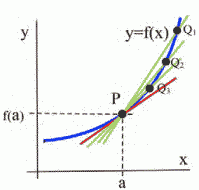
\includegraphics{img/chap2/image112.png}
    \caption{Secant lines approaching a tangent line.}
\label{fig:2-2-secants}
    \vspace{-10pt}
\end{wrapfigure}

To develop our formal definition of a tangent line, we consider the plot in Figure \ref{fig:2-2-secants}. In the plot, the red line is the tangent line of the curve $y=f(x)$ at the point $P = (a, f(a))$ and the green lines are secant lines that go through $P$. The closer the point $Q$ is to the point $P$, the closer the secant line slope gets to the tangent line slope and the closer the secant line gets to the tangent line. This will be key to finding the tangent slope, but first we need to more carefully define the idea of ``getting closer to.'' This will be done in Sections \ref{sec:limits} and \ref{sec:algderiv}.

This is an example for the reader to try.
\begin{example}
The graph in Figure \ref{fig:2-2-curve-for-tangents} is the graph of $y=f(x)$. We want to find the slope of the tangent line of this curve at the point $(1, 2)$.
\begin{figure}[!ht]
  \centering
    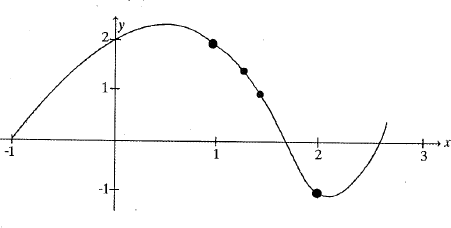
\includegraphics[width=0.6\textwidth]{img/chap2/image005.png}
    \caption{$y=f(x)$}
    \label{fig:2-2-curve-for-tangents}
\end{figure}

\begin{solution}
First, draw the secant line between the points $(1, 2)$ and $(2, -1)$ and compute its slope. Now draw the secant line between the points $(1, 2)$ and $(1.5, 1)$ and compute its slope. Compare the two lines you have drawn. Which would be a better approximation of the tangent line to the curve at the point $(1, 2)$?

Now draw the secant line between the points $(1, 2)$ and $(1.3, 1.5)$ and compute its slope. Is this line an even better approximation of the tangent line? Now draw your best guess for the tangent line and measure its slope. Do you see a pattern in the slopes?

You should have noticed that as the interval got smaller and smaller, the secant line got closer to the tangent line and its slope got closer to the slope of the tangent line. That's good news! We know how to find the slope of a secant line.
\end{solution}
\end{example}

In some applications, we need to know where the graph of a function $f(x)$ has horizontal tangent lines\index{Tangent line!horizontal}, that is, where the slope of the curve, or the rate of change of the function, is $0$.

\begin{example}
The graph of $y=g(x)$ is in Figure \ref{fig:2-2-gx}. At what values of $x$ does the graph of $g(x)$ have horizontal tangent lines?
\begin{figure}[!ht]
  \centering
    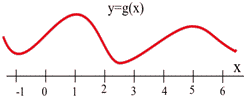
\includegraphics[width=0.4\textwidth]{img/chap2/image006.png}
    \caption{$y=g(x)$}
    \label{fig:2-2-gx}
\end{figure}

\begin{solution}
The tangent lines to the graph of $g(x)$ are horizontal when $x\approx -1,1,2.5,$ and $5$.
\end{solution}\end{example}

\subsection{Example: Instantaneous Velocity} 
To give another example of the concept of instantaneous rate of change, we consider the well-known and well-understood example of velocity. In fact, it was the problem of computing instantaneous velocity that led to the invention of calculus.

Suppose we drop a tomato from the top of a 100 foot building and time its fall.
\begin{wrapfigure}{R}{0.5\textwidth}
  \vspace{  0pt}
    \centering
    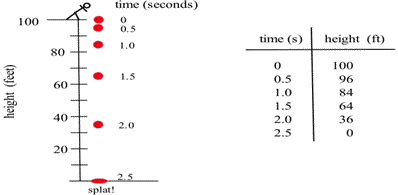
\includegraphics{img/chap2/image003.png}
    \caption{The height of a dropped tomato versus time.}
\label{fig:2-2-tomato}
\end{wrapfigure}

Some questions are easy to answer directly from the table.
\begin{example}
    \begin{itemize}
    \item[(a)] How long did it take for the tomato to drop 100 feet?

    \begin{solution}
    It took 2.5 seconds for the tomato to drop 100 feet.
    \end{solution}

    \item[(b)] How far did the tomato fall during the first second?

    \begin{solution}
    The tomato fell $100-84=16$ feet during the first second.
    \end{solution}

    \item[(c)] How far did the tomato fall during the last second?

    \begin{solution}
    The tomato fell $64-0=64$ feet during the last second.
    \end{solution}

    \item[(d)] How far did the tomato fall between $t=0.5$ and $t=1$ seconds? 

    \begin{solution}
    The tomato fell $96 - 84 = 12$ feet between $t=0.5$ and $t=1$ seconds.
    \end{solution}
    \end{itemize}
\end{example}
Some questions require a little calculation.
\begin{example}
    \begin{itemize}
    \item[(e)] What was the average velocity of the tomato during its fall?

    \begin{solution}
    Average velocity $= \frac{\mbox{change in position}}{\mbox{change in time}} = \frac{0-100 \mbox{ ft}}{2.5-0 \mbox{ s}} = -40 \mbox{ ft/s}$.
    \end{solution}

    \item[(f)] What was the average velocity between $t=1$ and $t=2$ seconds?

    \begin{solution}
    Average velocity $= \frac{\mbox{change in position}}{\mbox{change in time}} = \frac{36-84 \mbox{ ft}}{2-1 \mbox{ s}} = -48 \mbox{ ft/s}$.
    \end{solution}
    \end{itemize}
\end{example}

Now, we consider a different question that is an example of an instantaneous rate of change, and an example of a question that is significantly different from the previous example about average velocity.
\begin{example}
    How fast was the tomato falling one second after it was dropped?

    \begin{solution}
    Here we want the instantaneous velocity, the velocity at an instant in time. Unfortunately, the tomato is not equipped with a speedometer so we will have to give an approximate answer.

    One crude approximation of the instantaneous velocity after one second is simply the average velocity during the entire fall: $-40$ ft/s. However, the tomato fell slowly at the beginning and rapidly near the end so this estimate may or may not be a good answer.

    We can get a better approximation of the instantaneous velocity at $t=1$ by calculating the average velocities over a short time interval near $t=1$. The average velocity between $t=0.5$ and $t=1$ is $\displaystyle\frac{-12 \mbox{ feet}}{0.5 \mbox{ s}} = -24$ ft/s, and the average velocity between $t=1$ and $t=1.5$ is $\displaystyle\frac{-20 \mbox{ feet}}{0.5 \mbox{ s}} = -40$ ft/s, so we can be reasonably sure that the instantaneous velocity is between $-24$ ft/s and $-40$ ft/s.

    Another approximation would be by calculating the average velocity between $t=0.5$ and $t=1.5$, that is, the shortest time interval we have with $t=1$ in the middle: $\displaystyle\frac{64-96 \mbox{ feet}}{1.5-0.5 \mbox{ s}} = -32$ ft/s.

     Now, in general, the shorter the time interval over which we calculate the average velocity, the better the average velocity will approximate the instantaneous velocity. Using just the table in Figure \ref{fig:2-2-tomato}, we cannot find any shorter time interval. However, with a model or a function describing the height of the tomato, we could get a better approximation. We will plot the points and fit a curve to it and work from there.

    Notice that the data, plotted in Figure \ref{fig:2-2-tomato-model}, is not linear and has the same concavity (concave down), so a quadratic model may be appropriate. In fact, we know from physics that in the absence of air resistance, that a quadratic model would fit this kind of data perfectly. From LibreOffice, we can obtain the model
$$h(t) = 100 - 16t^2 \mbox{ feet after } t \mbox{ seconds}$$
for the height of the tomato. We plot this and the data together.

\begin{figure}[!ht]
    \centering
    \begin{subfigure}[b]{0.4\textwidth}

    \begin{tikzpicture}[scale=2]
    \def\xmin{0}
    \def\xmax{2.5}
    \def\xscale{1}

    \def\ymin{0}
    \def\ymax{100}
    \def\yscale{40}

    % grid
    \draw[step=0.5, very thin, gray] (0, 0) grid (2.5, 2.5);

    % axes
    \draw[->] (-0.2,0) -- coordinate (x axis mid) (2.7, 0) node[right] {$t$};
    \draw[->] (0,-0.2) -- coordinate (y axis mid) (0, 2.7) node[above] {$y$};

    % ticks
    \foreach \x in {0.5, 1, ..., 2.5}
     		\draw (\x,1pt) -- (\x,-3pt)
			node[anchor=north] {\x};
    	\foreach \y in {20, 40, ..., 100}
     		\draw (1pt,\y/\yscale) -- (-3pt,\y/\yscale) 
     			node[anchor=east] {\y}; 

    % labels
    \node[below = 15] at (x axis mid) {Time (seconds)};
	\node[rotate=90, above = 25] at (y axis mid) {Height (feet)};

    % plot 
    
    % points
    \foreach \pt in {(0, 100/\yscale), (0.5, 96/\yscale), (1, 84/\yscale), (1.5, 64/\yscale), (2, 36/\yscale), (2.5,0/\yscale)}
        \filldraw[color=aldRed] \pt circle [radius=2pt]; 
    % legend

    \end{tikzpicture}
    \caption{Data of the height of the tomato.}
    \end{subfigure}
    ~
    \begin{subfigure}[b]{0.4\textwidth}

    \begin{tikzpicture}[scale=2]
    \def\xmin{0}
    \def\xmax{2.5}
    \def\xscale{1}

    \def\ymin{0}
    \def\ymax{100}
    \def\yscale{40}

    % grid
    \draw[step=0.5, very thin, gray] (0, 0) grid (2.5, 2.5);

    % axes
    \draw[->] (-0.2,0) -- coordinate (x axis mid) (2.7, 0) node[right] {$t$};
    \draw[->] (0,-0.2) -- coordinate (y axis mid) (0, 2.7) node[above] {$y$};

    % ticks
    \foreach \x in {0.5, 1, ..., 2.5}
     		\draw (\x,1pt) -- (\x,-3pt)
			node[anchor=north] {\x};
    	\foreach \y in {20, 40, ..., 100}
     		\draw (1pt,\y/\yscale) -- (-3pt,\y/\yscale) 
     			node[anchor=east] {\y}; 

    % labels
    \node[below = 15] at (x axis mid) {Time (seconds)};
	\node[rotate=90, above = 25] at (y axis mid) {Height (feet)};

    % plot 
    \draw[smooth, samples=1000, domain=0:2.5, very thick, color=aldBlue] plot(\x,{(100-16*\x^2)/\yscale});    

    % points
    \foreach \pt in {(0, 100/\yscale), (0.5, 96/\yscale), (1, 84/\yscale), (1.5, 64/\yscale), (2, 36/\yscale), (2.5,0/\yscale)}
        \filldraw[color=aldRed] \pt circle [radius=2pt]; 
    % legend

    \end{tikzpicture}
    \caption{Modeling the height of the tomato.}
    \end{subfigure}
    \caption{ }
    \label{fig:2-2-tomato-model}
\end{figure}

Now we can approximate the velocity of the tomato at $t=1$ seconds by going off the model. We often use the symbol $\Delta$ (delta)\index{Delta} to indicate a finite difference between two values of a variable. In this context, $\Delta t$ is a difference in time and $\Delta h$ is a difference in the function $h$, i.e., a difference in height. With this notation, the average velocity over some time interval is $\frac{\Delta h}{\Delta t}$. In this example, 
$$\Delta h = h(1+\Delta t) - h(1) \enspace .$$
\begin{table}[ht!]
\begin{centering}
\begin{tabular}{lll}
\toprule
$\Delta t$ (seconds) & $\Delta h = h(1+\Delta t)-h(1)$ (feet) & $\frac{\Delta h}{\Delta t}$ (ft/s) \\
\midrule
1       & $h(2) - h(1) = 36-84 = -48$                   & $\dfrac{-48\mathstrut}{1\mathstrut} = -48$ \\
0.5     & $h(1.5) - h(1) = 64-84 = -20$                 & $\dfrac{-20\mathstrut}{0.5\mathstrut} = -40$ \\
0.1     & $h(1.1) - h(1) = 80.64-84 = -3.36$            & $\dfrac{-3.36\mathstrut}{0.1\mathstrut} = -33.6$ \\
0.01    & $h(1.01) - h(1) = 83.6784-84 = -0.3216$       & $\dfrac{-0.3216\mathstrut}{0.01\mathstrut} = -32.16$ \\
0.001   & $h(1.001) - h(1) = 83.967984-84 = -0.032016$  & $\dfrac{-0.032016\mathstrut}{0.001\mathstrut} = -32.016$ \\
\bottomrule
\end{tabular}
\caption{Average velocities approaching the instantaneous velocity at $t=1$ seconds.}
\label{tab:2-2-tomato-velocity}
\end{centering}
\end{table}
From the data in Table \ref{tab:2-2-tomato-velocity}, the average velocities are approaching $-32$ feet per second, which is in fact the (instantaneous) velocity of the tomato one second after being dropped.
\end{solution}
\end{example}

\subsection*{Example: Marginal Cost} 
\label{ssec:marginalcost}
Another example of the application of secant and tangent lines is {\bf marginal cost}\index{Marginal cost}\index{Cost!marginal}. 
\begin{definition}
    The {\bf marginal cost} at $q$ items, $MC(q)$, is the cost of producing the next item:
$$MC(q)=C(q+1)-C(q) \enspace .$$

In many cases, though, it's easier to approximate this difference using tangent lines, as the instantaneous rate of change of $C(n)$ at $n=q$. Some sources define the marginal cost this way. In this course, we will use both of these definitions as if they were interchangeable.
\end{definition} 
In other words, the marginal cost of $n$ items is the slope of the secant line of $y=C(n)$ through the points $(n, C(n))$ and $(n+1, C(n+1))$, but it can be approximated by the slope of the tangent line of $y=C(n)$ through the point $(n, C(n))$. 
\begin{example}
Table \ref{tab:2-2-cost} shows the total cost ($C(n)$) of producing $n$ items.
\begin{table}[ht!]
\centering
\begin{tabular}{cc}
\toprule
Items ($n$)	& Cost $C(n)$ \\
\midrule
0	& \$20,000\\
100	& \$35,000\\
200	& \$45,000\\	
300	& \$53,000\\
\bottomrule
\end{tabular}
\caption{Cost to produce $n$ items.}
\label{tab:2-2-cost}
\end{table}

When 200 items are made, estimate the marginal cost.

\begin{solution}
Since we don't have $C(201)$, We need to estimate the value of $MC(200)$ by estimating the slope of the tangent line at $n=200$ using secant lines. The secant line from $n=100$ to $n=200$ has a slope of:
$$MC(200) \approx \frac{\$45,000-\$35,000}{200-100 \mbox{ items}} = \$100 \mbox{ per item} \enspace .$$
The secant line from $n=200$ to $n=300$ has a slope of:
$$MC(200) \approx \frac{\$53,000-\$45,000}{300-200 \mbox{ items}} = \$80 \mbox{ per item} \enspace .$$

We could estimate the tangent slope by averaging these secant slopes, giving us an estimate of $\$90$ per item. 

Alternatively, we could estimate $MC(2000$ by finding the slope of the secant line between $n=100$ and $n=300$:
$$MC(200) \approx \frac{\$53,000-\$35,000}{300-100 \mbox{ items}} = \$90 \mbox{ per item} \enspace .$$

This tells us that after 200 items have been made, it will cost about $\$90$ to make one more item.
    \end{solution}
\end{example}


%Instantaneous velocity is an example of the instantaneous rate of change of a function, specifically position as a function of time. Therefore, we are interested in the more general concept of the instantaneous rate of change of a function.
%The average velocity over a time interval is ΔpositionΔtime, which is the slope of the secant line through two points on the graph of height versus time. The instantaneous velocity at a particular time and height is the slope of the tangent line to the graph at the point given by that time and height.
%
%graph
%Average vs Instantaneous Velocity
%Average velocity = ΔpositionΔtime = slope of the secant line through 2 points.
%
%Instantaneous velocity = slope of the line tangent to the graph.
%
%Growing Bacteria
%Suppose we set up a machine to count the number of bacteria growing on a Petri plate. At first there are few bacteria so the population grows slowly. Then there are more bacteria to divide so the population grows more quickly. Later, there are more bacteria and less room and nutrients available for the expanding population, so the population grows slowly again. Finally, the bacteria have used up most of the nutrients, and the population declines as bacteria die.
%
% bacteria 1
%The population graph can be used to answer a number of questions.
%
%What is the bacteria population at time t=3 days?
%
%From the graph, at t=3, the population is about 0.5 thousand, or 500 bacteria.
%
%What is the population increment from t=3 to t=10 days?
%
%At t=10, the population is about 4.5 thousand, so the increment is about 4000 bacteria.
%
%What is the rate of population growth from t=3 to t=10 days?
%
%The rate of growth from t=3 to t=10 is the average change in population during that time:
%average change in population ===\approx   change in populationchange in timeΔpopulationΔtime4000 bacteria7 days570 bacteria/day.
%This is the slope of the secant line through the two points (3, 500) and (10, 4500).
%
%What is the rate of population growth on the third day, at t=3 ?
%
%This question is asking for the instantaneous rate of population change, the slope of the line which is tangent to the population curve at (3, 500). If we sketch a line approximately tangent to the curve at (3, 500) and pick two points near the ends of the tangent line segment , we can estimate that instantaneous rate of population growth is approximately 320 bacteria/day .
%
% bacteria 2

%Let's explore further this idea of finding the tangent slope based on the secant slope.

%\begin{example}
%Find the slope of the line $L$ in the graph below which is tangent to $f(x)=x^2$ at the point $(2,4)$.
%
%\begin{solution} We could estimate the slope of L from the graph, but we won't. Instead, we will use the idea that secant lines over tiny intervals approximate the tangent line.
%
%graphgraph
%We can see that the line through (2,4) and (3,9) on the graph of f is an approximation of the slope of the tangent line, and we can calculate that slope exactly: m=ΔyΔx=9-43-2=5. But m=5 is only an estimate of the slope of the tangent line and not a very good estimate. It's too big. We can get a better estimate by picking a second point on the graph of f which is closer to (2,4) - the point (2,4) is fixed and it must be one of the points we use.
%
%From the second figure, we can see that the slope of the line through the points (2,4) and (2.5,6.25) is a better approximation of the slope of the tangent line at (2,4): m=ΔyΔx=6.25-42.5-2=2.250.5=4.5, a better estimate, but still an approximation. We can continue picking points closer and closer to (2,4) on the graph of f, and then calculating the slopes of the lines through each of these points and the point (2,4):
%
%Points to the left of (2,4)
%x	y=x2	Slope of line through (x,y) and (2,4).	1.5	2.25	3.5	1.9	3.61	3.9	1.99	3.9601	3.99
%Points to the right of (2,4)
%x	y=x2	Slope of line through (x,y) and (2,4).	3	9	5	2.5	6.25	4.5	2.01	4.0401	4.01
%The only thing special about the x-values we picked is that they are numbers which are close, and very close, to x=2. Someone else might have picked other nearby values for x. As the points we pick get closer and closer to the point (2,4) on the graph of y=x2, the slopes of the lines through the points and (2,4) are better approximations of the slope of the tangent line, and these slopes are getting closer and closer to 4.
%
%We can bypass much of the calculating by not picking the points one at a time: let's look at a general point near (2,4). Define x=2+h so h is the increment from 2 to x. If h is small, then x=2+h is close to 2 and the point (2+h,f(2+h))=(2+h,(2+h)2) is close to (2,4). The slope m of the line through the points (2,4) and (2+h,(2+h)2) is a good approximation of the slope of the tangent line at the point (2,4):
%
%graph
%m=(2+h)2-4(2+h)-2=(4+4h+h2)-4h=4h+h2h=h(4+h)h=4+h
%The value m=4+h is the slope of the secant line through the two points (2,4) and (2+h,(2+h)2). As h gets smaller and smaller, this slope approaches the slope of the tangent line to the graph of f at (2,4).
%
%More formally, we could write:
%Slope of the tangent line=ΔyΔx=limh→0(4+h).
%We can easily evaluate this limit using direct substitution, finding that as the interval h shrinks towards 0, the secant slope approaches the tangent slope, 4.
%\end{solution}\end{example}
%
%The tangent line problem and the instantaneous velocity problem are the same problem. In each problem we wanted to know how rapidly something was changing at an instant in time, and the answer turned out to be finding the slope of a tangent line, which we approximated with the slope of a secant line. This idea is the key to defining the slope of a curve.

\subsection{Exercises}
\label{2-2-exercies}

\begin{enumerate}
\item	What is the slope of the line through the points $(3,9)$  and  $(x, y)$  for $y = x^2$ and:
    \begin{itemize}
    \item[(a)] $x = 2.97$?   
    \item[(b)] $x = 3.001$?   
	\item[(c)] $x = 3+h$?   
    \item[(d)] What happens to this last slope when $h$  is very small (close to 0)?   
    \item[(e)] Sketch the graph of $y = x^2$  for  $x$  near  $3$.
    \end{itemize}

\item	What is the slope of the line through  the points $(-2,4)$  and  $(x, y)$  for $y = x^2$  and:
    \begin{itemize}
    \item[(a)] $x = -1.98$?   
    \item[(b)] $x = -2.03$?   
	\item[(c)] $x = -2+h$?   
    \item[(d)] What happens to this last slope when $h$  is very small (close to 0)?   
    \item[(e)] Sketch the graph of $y = x^2$  for  $x$  near  $-2$.
    \end{itemize}    
 
\item	What is the slope of the line through  the points $(2,4)$  and  $(x, y)$  for $y = x^2 + x - 2$   and  
\begin{itemize}
    \item[(a)] $x = 1.99$?   
    \item[(b)] $x = 2.004$?   
	\item[(c)] $x = 2+h$?   
    \item[(d)] What happens to this last slope when $h$  is very small (close to 0)?   
    \item[(e)] Sketch the graph of $y = x^2+x-2$  for  $x$  near  $2$.
    \end{itemize} 

\item	What is the slope of the line through the points $(-1,-2)$  and  $(x, y)$  for $y = x^2 +x - 2$  and:
\begin{itemize}
    \item[(a)] $x = -0.98$?   
    \item[(b)] $x = -1.03$?   
	\item[(c)] $x = -1+h$?   
    \item[(d)] What happens to this last slope when $h$  is very small (close to 0)?   
    \item[(e)] Sketch the graph of $y = x^2+x-2$  for  $x$  near  $-1$.
    \end{itemize} 

\begin{minipage}{\linewidth}
\begin{wrapfigure}{r}{0.4\textwidth}
    \centering
    \vspace{-12pt}
    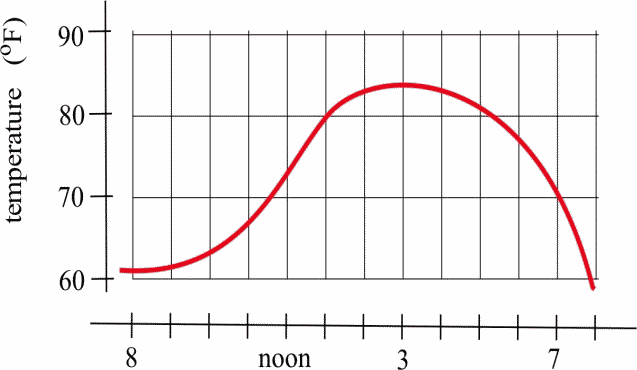
\includegraphics[width=0.4\textwidth]{img/chap2/image007.png}
    \caption{Temperature in Ames.}
    \label{fig:2-2-exer5}
\end{wrapfigure}

\item	The graph in Figure \ref{fig:2-2-exer5} shows the temperature during a day in Ames.
    \begin{itemize}
    \item[(a)] What was the average rate of change in temperature from  9 am  to  1 pm? 
    \item[(b)] Sketch a tangent line on the curve and estimate how fast the temperature was changing at  10 am.  
    \item[(c)] Sketch a tangent line on the curve and estimate how fast the temperature was changing at 7 pm.
    \end{itemize}
\end{minipage}

\begin{minipage}{\linewidth}
\begin{wrapfigure}{r}{0.4\textwidth}
    \centering
    %\vspace{-12pt}
    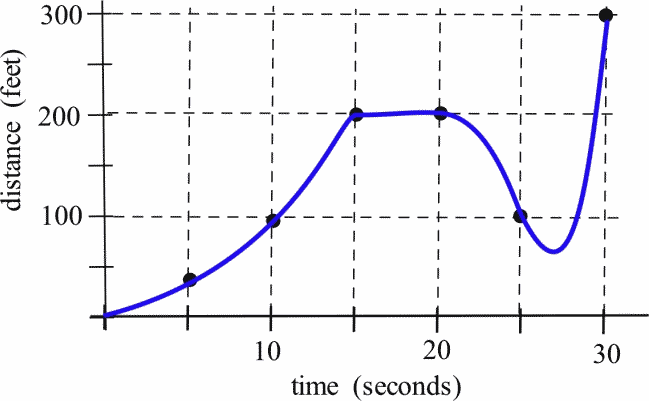
\includegraphics[width=0.4\textwidth]{img/chap2/image008.png}
    \caption{Net distance a car has traveled.}
    \label{fig:2-2-exer6}
\end{wrapfigure}

\item	The graph in Figure \ref{fig:2-2-exer6} shows the distance of a car from a measuring position located on the edge of a straight road.
    \begin{itemize}
    \item[(a)]	 What was the average velocity of the car from  $t = 0$  to  $t = 30$ seconds?
    \item[(b)]	What was the average velocity of the car from  $t = 10$  to  $t = 30$ seconds?
    \item[(c)]	Sketch a tangent line on the curve and estimate the velocity of the car at  $t = 10$, at $t = 20$, and at $t = 30$ seconds.
    \item[(d)]	What does the horizontal part of the graph between  $t = 15$  and  $t = 20$ seconds mean?
    \item[(e)]	What does the negative velocity at  $t = 25$  represent?
    \end{itemize}
\end{minipage}

\begin{minipage}{\linewidth}
\begin{wrapfigure}{r}{0.4\textwidth}
    \centering
    \vspace{-12pt}
    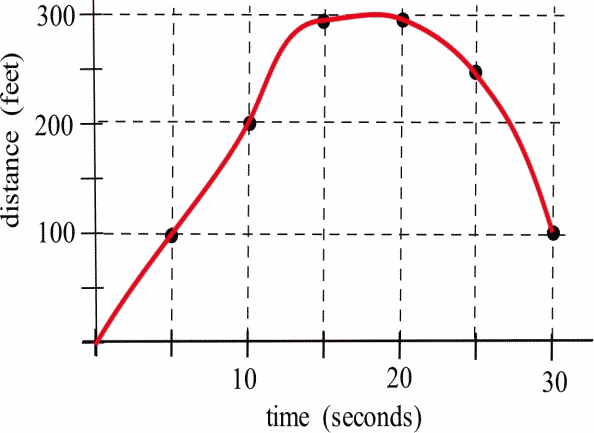
\includegraphics[width=0.4\textwidth]{img/chap2/image009.png}
    \caption{Net distance a car has traveled.}
    \label{fig:2-2-exer7}
\end{wrapfigure}

\item	The graph in Figure \ref{fig:2-2-exer7} shows the distance of a car from a measuring position located on the edge of a straight road.
    \begin{itemize}
    \item[(a)]	What was the average velocity of the car from  $t = 0$  to  $t = 20$ seconds?
    \item[(b)]	What was the average velocity from  $t = 10$  to  $t = 30$ seconds?
    \item[(c)]	About how fast was the car traveling at  $t = 10$ 
		seconds?  at  $t = 20$ seconds?  at  $t = 30$ seconds?
    \end{itemize}
\end{minipage}

\begin{minipage}{\linewidth}
\begin{wrapfigure}{r}{0.4\textwidth}
    \centering
    %\vspace{-12pt}
    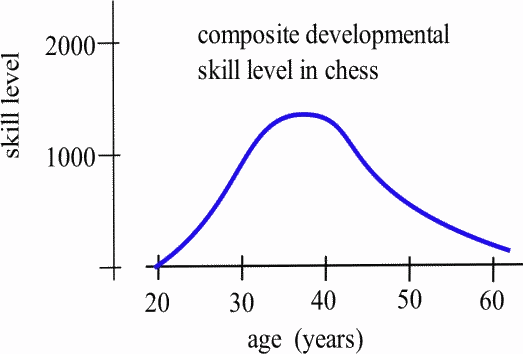
\includegraphics[width=0.4\textwidth]{img/chap2/image010.png}
    \caption{Developmental skill level of chess masters versus age.}
    \label{fig:2-2-exer8}
\end{wrapfigure}

\item	The graph in Figure \ref{fig:2-2-exer8} shows the composite developmental skill level of chess masters at different ages as determined by their performance against other chess masters.  (From {\em Rating Systems for Human Abilities}, by W.H.\ Batchelder and R.S.\ Simpson, 1988.\ UMAP Module 698.)
\begin{itemize}
    \item[(a)]	At what age is the ``typical'' chess master playing the best chess?
    \item[(b)]	At approximately what age is the chess master's skill level increasing most rapidly?
    \item[(c)]	Describe the development of the ``typical'' chess master's skill in words.
    \item[(d)]	Sketch graphs which you think would reasonably describe the performance levels versus age for an athlete, a classical pianist, a rock singer, a mathematician, and a professional in your major field.
\end{itemize}
\end{minipage}
\end{enumerate}
